\section{Длины: кто промахивается и насколько}\label{sec:lengths}

\begin{proposition}\label{prop:lengths}
При $0<\theta<\pi$ выполнено $C<A<T$, и
\[
A-C=\tfrac{1}{24}\theta^3+O(\theta^5),\qquad T-A=\tfrac{1}{12}\theta^3+O(\theta^5).
\]
В главном порядке избыток внешнего пути ровно вдвое больше недостачи хорды. Следовательно,
\[
\frac{2C+T}{3}=\theta+\tfrac{1}{320}\theta^5+O(\theta^7),
\]
и $(2C+T)/3>\theta$ на всём интервале (неравенство Снеллиуса~--- Гюйгенса
$2\sin x+\tan x>3x$ при $0<x<\pi/2$, где $x=\theta/2$).
\end{proposition}
\begin{proof}
Ряды следуют из $\sin x=x-x^3/6+x^5/120-\dots$ и $\tan x=x+x^3/3+2x^5/15+\dots$ при
$x=\theta/2$. Неравенства классические \cite{archimedes,huygens}; все они проверены скриптом
\texttt{verify.py}.
\end{proof}

\begin{plain}
Короткий путь напрямик недотягивает до истинного пути, а обход перелетает. Для малых поворотов
перелёт всегда ровно вдвое больше недолёта. Поэтому если взять путь напрямик дважды, а
обход один раз и усреднить, обе ошибки сократятся, и получится истинная длина почти
идеально: оставшаяся ошибка убывает как пятая степень угла. Снеллиус нашёл это в 1621 году,
а Гюйгенс доказал в 1654-м. Ни одна из сторон в одиночку не говорит правды; а вместе~---
почти правду.
\end{plain}

\begin{figure}[t]\centering
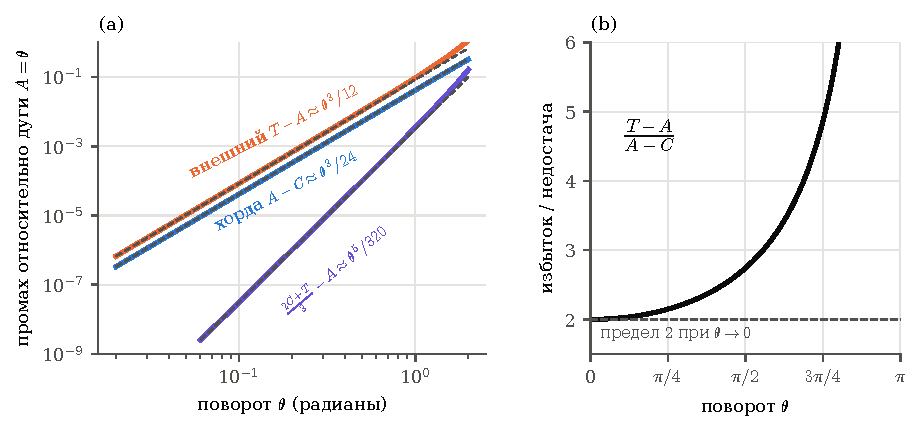
\includegraphics[width=\linewidth]{figures/fig_lengths.pdf}
\caption{Длины. \textbf{(a)} Недостача хорды $A-C$ и избыток внешнего пути
$T-A$ убывают как $\theta^3$, а именно как $\theta^3/24$ и $\theta^3/12$ (штриховые линии: главные члены из
предложения~\ref{prop:lengths}); смесь Снеллиуса~--- Гюйгенса $2{:}1$ убывает как
$\theta^5/320$. \textbf{(b)} Отношение избытка к недостаче равно $2$ в пределе и
растёт с ростом поворота; сокращение~--- утверждение о малых углах.}
\label{fig:lengths}
\end{figure}

\section{Поворот как число}\label{sec:number}

Будем понимать поворот как комплексное число $U=e^{i\theta}$. Тогда хорда~--- это комплексное
число $U-1$, и
\[
U-1=2i\sin(\theta/2)\,e^{i\theta/2}.
\]
Её длина равна $C$, а её направление~--- это начальное направление, повёрнутое на $\theta/2$ (плюс
четверть оборота). \emph{Хорда поворачивается вдвое медленнее отрезка.} Полный оборот
отрезка, $\theta=2\pi$, поворачивает направление хорды лишь на полуоборот.

\paragraph{Хорда и сходство.} Положим
\[
S=\cos^2(\theta/2)=\tfrac12(1+\operatorname{Re}U),\qquad d=\sin(\theta/2)=\tfrac12 C.
\]
Тогда $S+d^2=1$ и $1-S=C^2/4$. Это тождество из статьи о двойном накрытии
\cite{davis-dc}, где $d$ понимается как половина хорды, а $S$~--- как сходство двух
положений. Два положения полностью одинаковы ($S=1$), когда хорда обращается в нуль. Они
полностью различны ($S=0$) при полуобороте, когда хорда~--- диаметр.

\paragraph{Касательная и отображение Кэли.} Отрезок касательной $\tau=\tan(\theta/2)$ строит
поворот алгебраически, без экспоненты:
\[
U=\frac{1+i\tau}{1-i\tau},\qquad
\tau=\frac{\sin\theta}{1+\cos\theta}=\frac{\operatorname{Im}U}{1+\operatorname{Re}U}=
\frac{\operatorname{Im}U}{2S}.
\]
Это преобразование Кэли \cite{cayley}. При $\theta\to\pi$ имеем $\tau\to\infty$: при
полуобороте две касательные параллельны, никогда не пересекаются, и у внешнего пути нет
вершины. Отображение Кэли достигает любого поворота, кроме полуоборота.

\begin{plain}
Как число поворот~--- это точка на единичной окружности. Путь напрямик~--- это «где ты
сейчас минус где ты начинал». Его направление поворачивается вдвое медленнее палки, поэтому
один полный оборот палки поворачивает путь напрямик только на полуоборот. Половина длины
пути напрямик~--- это в точности расстояние $d$ в тождестве двойного накрытия $S+d^2=1$, так
что путь напрямик измеряет, насколько различны два положения. Отрезок обхода~--- то
единственное число, которое восстанавливает весь поворот одной арифметикой, без экспонент.
При полуобороте он ломается: две боковые линии параллельны и никогда не встречаются.
\end{plain}

\section{Энергия}\label{sec:energy}

В решёточной калибровочной теории поворот $U$~--- это голономия по границе грани, а энергия
грани измеряет, насколько $U$ далёк от $1$ \cite{wilson}. Каждый из трёх путей даёт
энергию:
\[
C^2=2(1-\cos\theta)=\theta^2-\tfrac{1}{12}\theta^4+\tfrac{1}{360}\theta^6-\dots,\qquad
A^2=\theta^2,\qquad
T^2=\theta^2+\tfrac16\theta^4+\tfrac{17}{720}\theta^6+\dots
\]
$C^2$~--- это действие Вильсона (с точностью до нормировки), а $A^2$~--- геодезическое
действие Мантона \cite{manton}, то есть континуальная энергия грани. Касательная энергия снова
промахивается с другой стороны, и снова ровно вдвое сильнее в главном порядке. Поэтому те же
веса Снеллиуса~--- Гюйгенса её сокращают.

\begin{proposition}\label{prop:energy}
\[
\frac{2C^2+T^2}{3}=\theta^2+\tfrac{7}{720}\theta^6+\tfrac{1}{1008}\theta^8+O(\theta^{10}).
\]
Член с $\theta^4$ сокращается точно. Эта комбинация алгебраична по $U$:
$C^2=|U-1|^2$ и $T^2=4\,|\operatorname{Im}U|^2/(1+\operatorname{Re}U)^2$.
\end{proposition}

\begin{plain}
Энергию поворота можно измерять по пути напрямик, по истинному пути или по обходу.
Решёточная физика с 1974 года пользуется путём напрямик, потому что его легко вычислять;
истинный путь~--- это то, что имеет в виду континуум. Энергия по пути напрямик чуть меньше,
чем нужно, а энергия по обходу чуть больше, причём вдвое сильнее. Смесь в пропорции два к
одному сокращает главную ошибку, и для этого нужна только арифметика над $U$.
\end{plain}

\begin{figure}[t]\centering
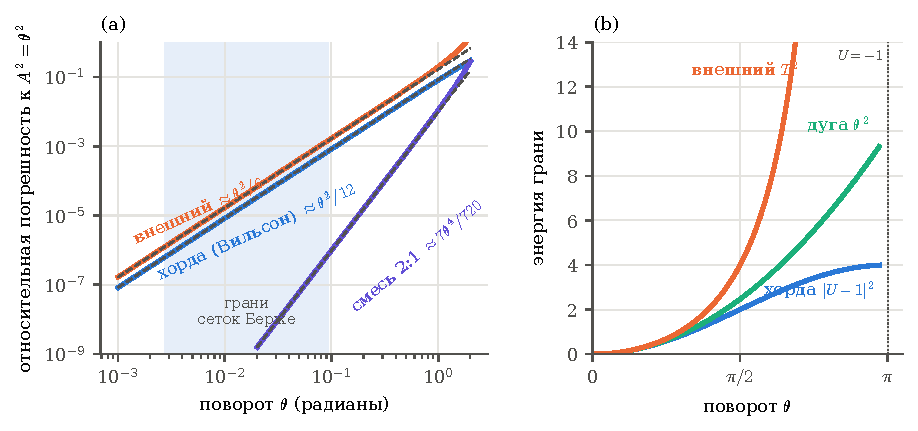
\includegraphics[width=\linewidth]{figures/fig_energy.pdf}
\caption{Энергия. \textbf{(a)} Относительная ошибка каждой энергии грани по сравнению с
континуальной энергией $\theta^2$: у хорды (действие Вильсона) она равна $\theta^2/12$, у внешнего
пути~--- $\theta^2/6$, у смеси $2{:}1$~--- $7\theta^4/720$ (предложение~\ref{prop:energy};
штриховые линии~--- главные члены). Затенённая полоса~--- диапазон углов граней на сетках
$SU(2)$ с метрикой Берже из раздела~\ref{sec:mesh}, от медианы при $n=5$ до наибольшего угла при $n=1$.
\textbf{(b)} Три энергии во всём диапазоне поворотов: энергия хорды ограничена числом $4$,
энергия дуги равна $\theta^2$, а у энергии внешнего пути есть барьер при $U=-1$.}
\label{fig:energy}
\end{figure}

\begin{remark}[Что это исправляет и чего не исправляет]
На решётке с шагом $a$ и для гладкого поля $\theta=O(a^2)$, так что член с $\theta^4$~--- это
относительная поправка порядка $a^4$. Главная решёточная ошибка имеет порядок $a^2$ и
происходит от формы грани, а не от компактности группы; именно её устраняет улучшение
Симанзика \cite{lw}. Приведённая выше комбинация затрагивает только ошибку компактности.
Эта ошибка существенна для сильных полей и грубых решёток и пренебрежимо мала для гладких
полей на мелких решётках. Кроме того, касательная энергия расходится при полуобороте $U=-1$,
в отличие от энергии Вильсона и подобно отображению Кэли. Решёточные действия ровно с таким
барьером изучались как действия, сохраняющие топологию \cite{luscher,fukaya}: они замораживают
топологию в методе Монте-Карло, а Кройц утверждал, что такие условия допустимости несовместимы с
положительностью трансфер-матрицы \cite{creutz}. Как этот барьер ведёт себя в моделировании для
смеси, здесь не исследуется.
\end{remark}

\section{Неабелев поворот}\label{sec:su2}

Единичный кватернион (элемент $SU(2)$) имеет вид $U=\cos a+n\sin a$, где $n$~--- чисто мнимый
единичный кватернион. Всё сказанное выше переносится на этот случай с заменой $\theta$ на
геодезический угол $a$ на $S^3$:
\[
|U-1|=2\sin(a/2),\qquad \log U=a\,n,\qquad
U=(1+v)(1-v)^{-1}\ \text{где}\ v=\frac{\operatorname{Im}U}{1+\operatorname{Re}U},\ |v|=\tan(a/2).
\]
Кватернион $U$ поворачивает трёхмерное пространство на угол $2a$, так что хорда, дуга и внешний
путь кватерниона живут на двойном накрытии описываемого им вращения. Вектор Кэли $v$
снова достигает всего, кроме $U=-1$~--- копии единицы на другом листе накрытия.
Скрипт \texttt{verify.py} проверяет все три формулы на $2{,}000$ случайных кватернионах. Хорда
и дуга совпадают с точностью до $10^{-14}$. Восстановление по Кэли совпадает с точностью до
$10^{-10}$; его число обусловленности растёт как $1/(1+\cos a)$ вблизи полуоборота.

\begin{plain}
Те же три пути существуют и для поворотов в трёх измерениях, записанных кватернионами.
Формулы те же самые, только угол поворота измеряется на трёхмерной сфере. Обход
по-прежнему восстанавливает поворот простой арифметикой и по-прежнему ломается только при
полуобороте.
\end{plain}

У вектора Кэли есть наглядный образ. Поскольку $v=\operatorname{Im}U/(1+\operatorname{Re}U)$,
это стереографическая проекция $U$ из точки $-1$ на экваториальное пространство
$\operatorname{Re}U=0$. Рисунок~\ref{fig:cayley} изображает её на одно измерение ниже, на $S^2$.

\begin{figure}[t]\centering
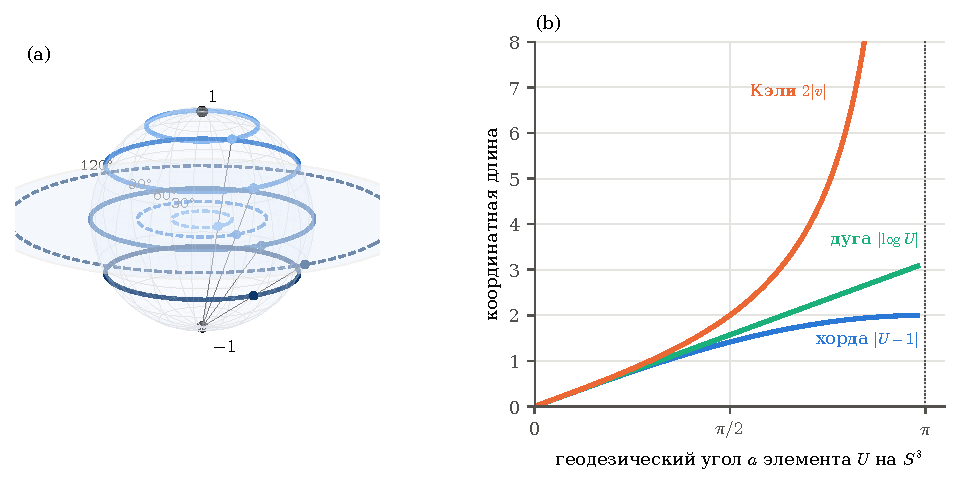
\includegraphics[width=\linewidth]{figures/fig_cayley_3d.pdf}
\caption{Вектор Кэли как стереографическая проекция, изображённая на $S^2$ вместо $S^3$.
\textbf{(a)} Вертикальная ось~--- $\operatorname{Re}U$. Сплошные окружности~--- повороты на
геодезический угол $a=30^\circ,60^\circ,90^\circ,120^\circ$ от $1$; штриховые окружности того же
оттенка~--- их образы Кэли в плоскости $\operatorname{Re}U=0$, радиуса $\tan(a/2)$. Тонкие
лучи исходят из точки проекции $-1$. При $a\to\pi$ образ уходит на бесконечность, поэтому
отображение Кэли достигает всего, кроме $U=-1$. \textbf{(b)} Три координаты одного
поворота: хорда $|U-1|=2\sin(a/2)$, дуга $|\log U|=a$ и координата Кэли $2|v|=2\tan(a/2)$. Это
длины $C$, $A$ и $T$ из раздела~\ref{sec:lengths}, прочитанные на $S^3$.}
\label{fig:cayley}
\end{figure}
